\documentclass{deliverablereport}

\deliverable{dissem}{ibook1}
\deliverydate{31/08/2018}
\duedate{31/08/2018 (M36)}
\author{Marcin Kostur, Jerzy Łuczka, Jan Aksamit, Jolanta Marzec}

\begin{document}
\maketitle

Linear Algebra and Nonlinear Processes in Biology are examples of
interactive capabilities

% \githubissuedescription

\section{Introduction}

Interactive webpages have always been an attractive tool in
education. It has started in the age of Adobe-Flash technology, when a
lot of educational materials have been created. The advent of
javascript has led to significant improvements in that field: in the
first place it created a possibility to author the content with Open
Source tools and secondly it increased the portability to practically
all devices equipped with modern web browser.

The problems which was persistent in those solutions was the big gap
between authoring of interactive tools and usage. Usually the code
behind of interactive examples was not very educational and was not
supposed to be edited by the target user. On the other hand Open
Source tools such as \Sage, delivered a versatile solution to this
problem.  The \texttt{@interact} decorator has made possibile to
convert a scientific calculation into web-based interactive
application. The biggest advantage of this solution is that one can
create a visually appealing scintific interaction using the same
environment in which the mathematical exlorations took place.


\section{Interactive book technology}

We have used well known in Python community sphinx documentation
generator for the main authoring tool. Sphinx contains plugins system,
which allows specialize it for a particular application. In our case
we will apply extenstion able to: 

\begin{itemize}
\item embedd \Sage code and allow for interactive execution on a
  remote server using SageMathCell  technology
\item use conditional compilation of parts depending e.g. if target medium is interactive of not.
\item include automatically \Jupyter notebooks with embedded output
\item  produce high quality  pdf via \LaTeX system.
\end{itemize}  


In the authoring process one can produce notebook (sagenb or \Jupyter
based) and decide if it should be included into the sphinx book or
choose selected examples and influde them as live SageCellServer code
which can be used interactively. It has to be stressed that not only
elemnents having \texttt{@interact} are usefull. Practically all 
excercises can be done inside the book in the interactive code
boxes. It is reasonable, however, to limit the reader to write only
short pieces of code in this way.  The code written in browser without
login is volatile and can dissappear if one reloads the page.

\begin{figure}
\centerline{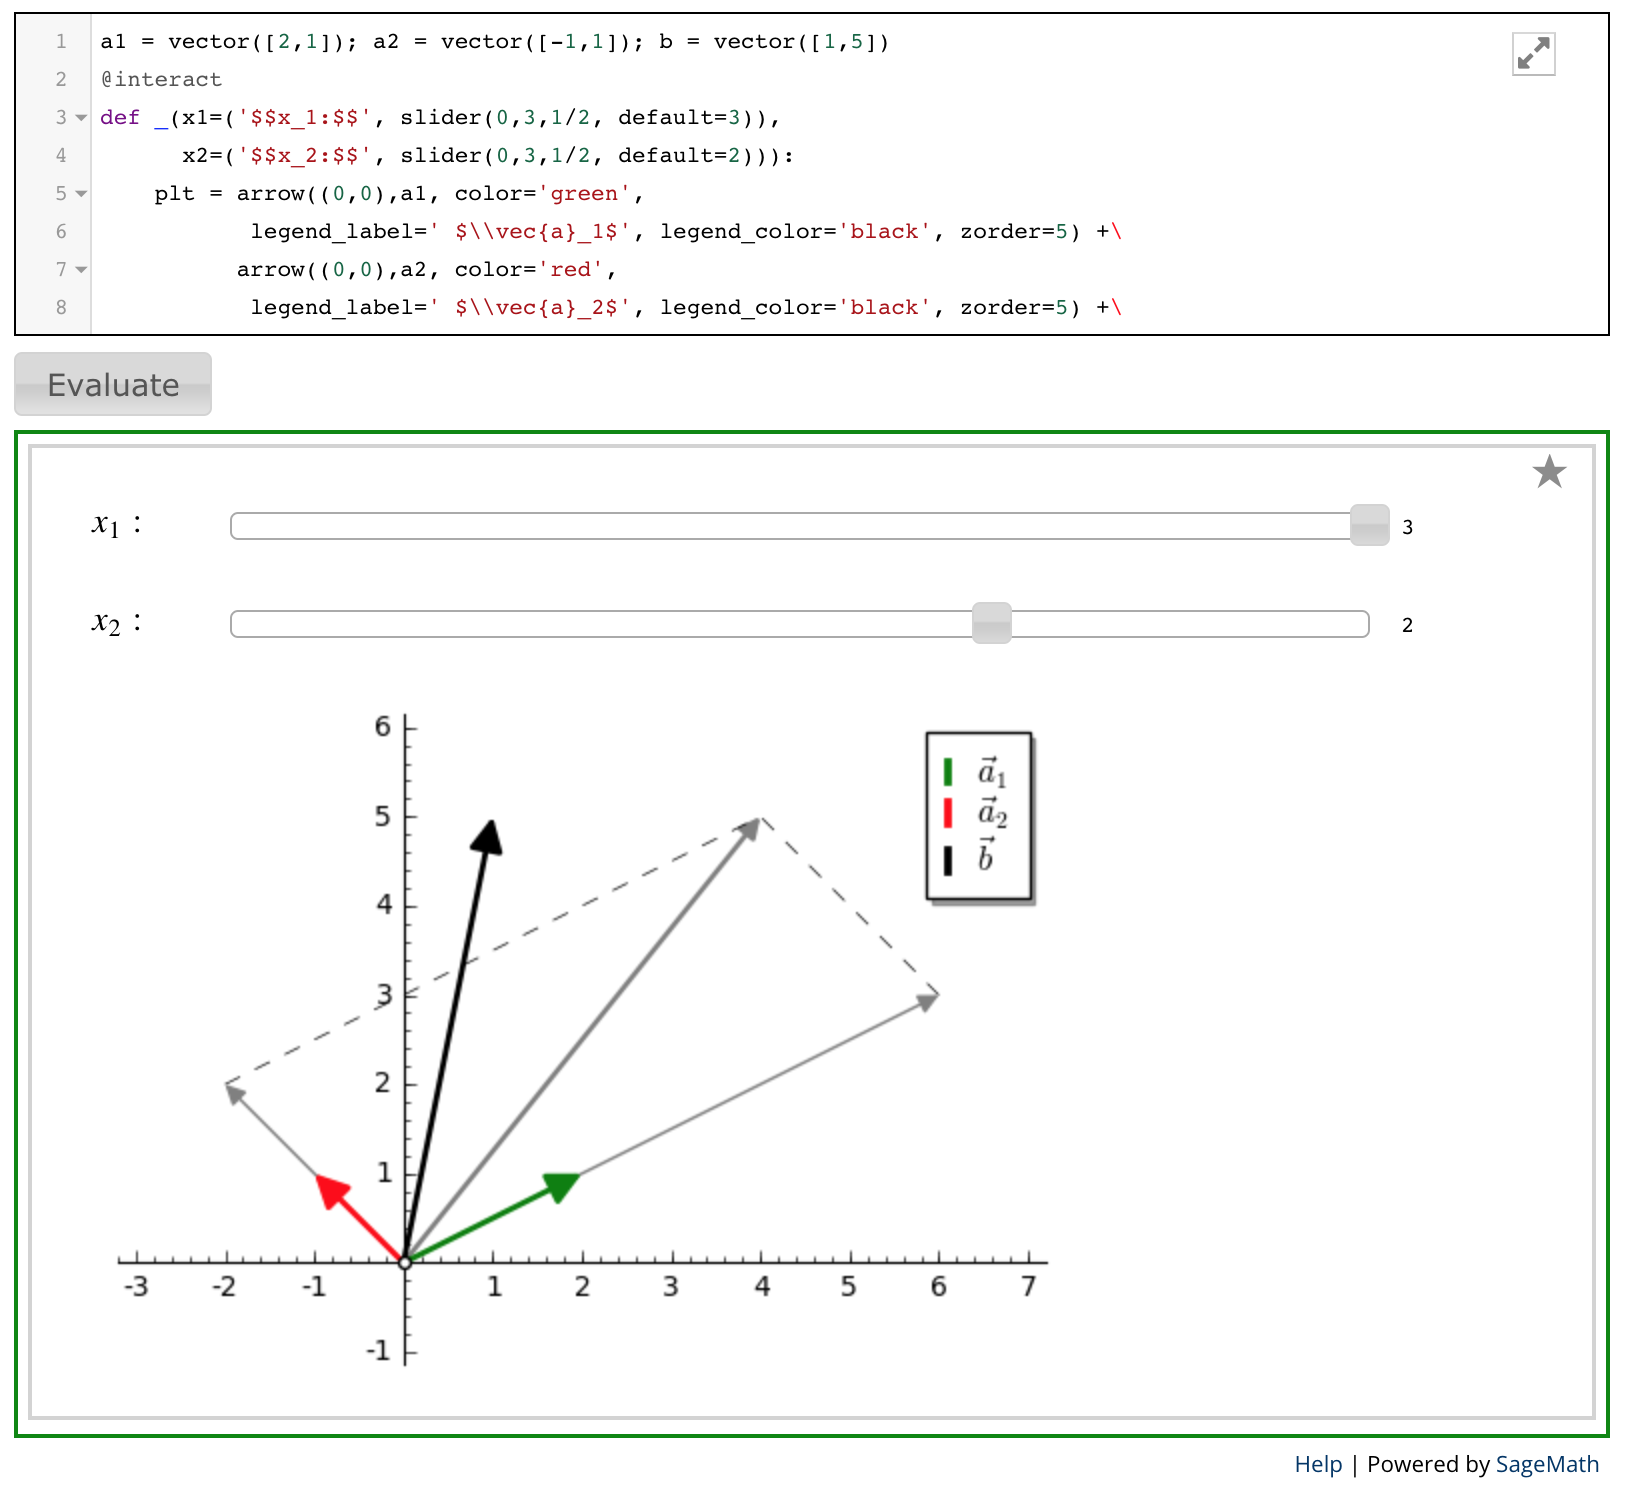
\includegraphics[width=1.0\textwidth]{interact_in_sphinx.png}}
\caption{\label{fig:jupyterdemo} An example of \texttt{@interact} in
  sphincs generated web version of interactive book. The upper box
  shows the code and the lower box shows the output.}
\end{figure}


\section{ Nonlinear Processes in Biology }

The book is in large extend based on coursework taught at University
of Silesia. It was primarily based on sagenb system and gradually was
converted into the interactive book with live examples.


The book covers the classical topics in modeling in
biology. Methodologically it can be split into following groups:

\begin{enumerate}
\item Qualitative methods in ODE. It include the analysis of the model
  properties depending on parameters, drawing a phase portraits,
  performing analysis of a linear stability of fix points of the
  system. This requires symbolic manipulations as well as certain
  techniques from numerical analysis like root finding. 
  
\item Numerical solving of ODEs. It is complementing
\item Numerical solving of PDE-s - diffusion equation,
  reaction-diffusion and similar. It requires good tools in data
  processing, usually uses numpy for calculations.
\item 
  
\end{enumerate}

\section{Lectures on Linear Algebra}

This book is based on courses of linear algebra for physics students
taught in recent years at the University of Silesia. It has been
gradually equipped with interactive materials. \Sage was used as a
tool for performing computations. 


\end{document}

%%% Local Variables:
%%% mode: latex
%%% TeX-master: t
%%% End:

